\documentclass[dvipdfmx]{jarticle}
\usepackage{graphicx}
\usepackage{amsmath}
\usepackage[top=30truemm,bottom=30truemm,left=25truemm,right=25truemm]{geometry}
\usepackage{listings,jvlisting}
\usepackage{amssymb}

\lstset{
  basicstyle={\ttfamily},
  identifierstyle={\small},
  commentstyle={\smallitshape},
  keywordstyle={\small\bfseries},
  ndkeywordstyle={\small},
  stringstyle={\small\ttfamily},
  frame={tb},
  breaklines=true,
  columns=[l]{fullflexible},
  numbers=left,
  xrightmargin=0zw,
  xleftmargin=3zw,
  numberstyle={\scriptsize},
  stepnumber=1,
  numbersep=1zw,
  lineskip=-0.5ex
}

\begin{document}

\begin{titlepage}
    \begin{center}
        \vspace*{60pt}
        {\LARGE プログラミングDレポート}
        \vspace*{240pt}\\
        \begin{tabular}{rl}
            担当教員 & 小南大智\\
            提出日 & \today\\
            氏名 & 山久保孝亮\\
            学籍番号 & 09B22084\\
            メールアドレス & u327468b@ecs.osaka-u.ac.jp
        \end{tabular}
    \end{center}
\end{titlepage}

\section{プログラムの操作方法と機能}
今回のライフゲームの課題はRunボタンが押されるとゲームが開始する.
私が作成した機能と操作方法は以下のとおりである.
\subsection{盤面の描画}
今回のライフゲームではゲームが開始した際にウィンドウが開き,そこにnext,undo,newgameのボタンとともに盤面が表示されるという仕様になっている.
生きている状態のセルを黒色,死んでいる状態のセルを灰色で表すこととした.最初はすべてのセルが死んでいる状態となっている.
また,盤面の縦と横の座標は以下の図1ような仕様とした.また,(i,j)と指定されると横軸がi,縦軸がjの行と列をそれぞれ考え,それらが交差するセルを表す.
\begin{figure}[h]
  \centering
  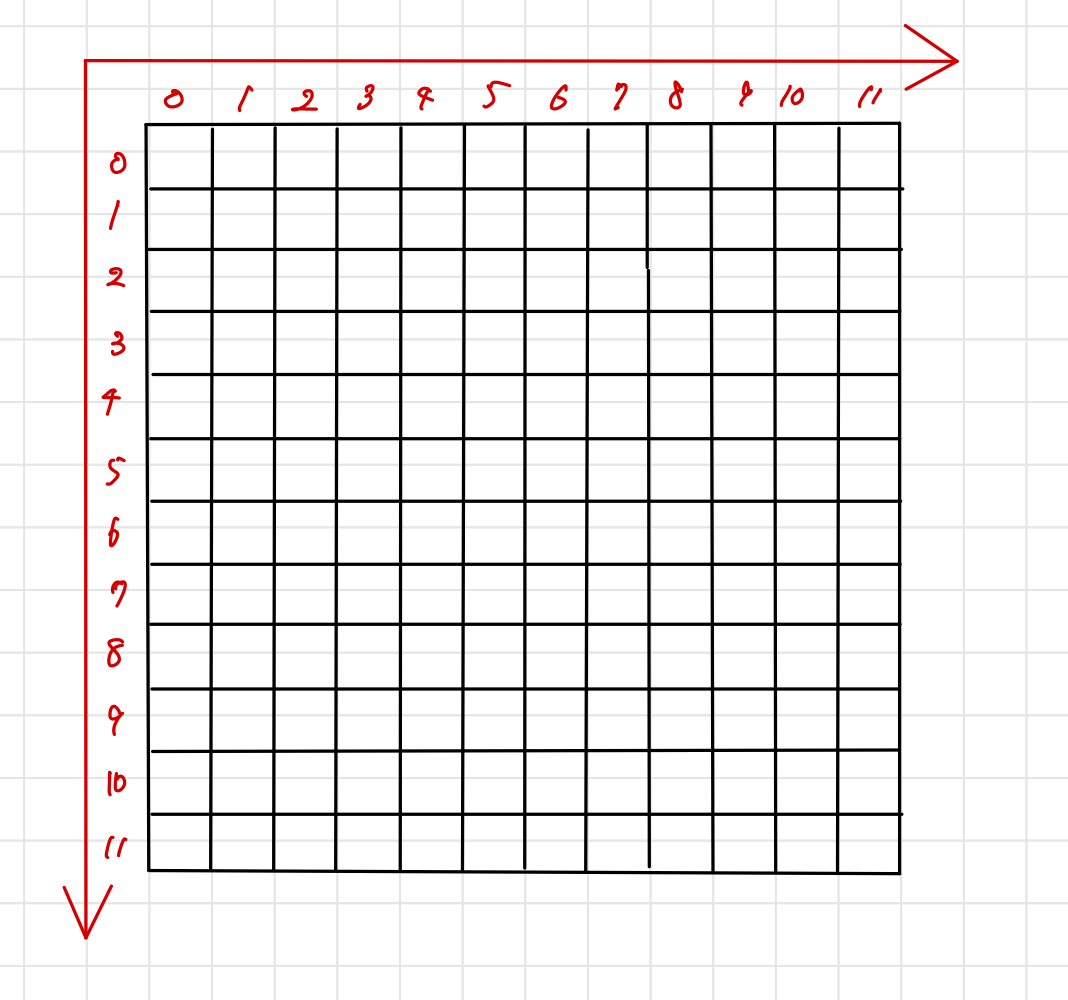
\includegraphics[width=6cm]{zahyou.png}
  \caption{座標の仕様}
\end{figure}
\subsubsection{ウィンドウのサイズ変更}
ウィンドウの大きさをユーザ側が変更した際にはその変更に合わせて盤面の大きさも変更される.盤面のサイズの初期値は縦300,横400ピクセルで最小値は縦200,横300ピクセルである.
以下の図2,3はウィンドウを極端に横に大きくしたときの例と縦に大きくしたときの例である.
\begin{figure}[htbp]
    \begin{minipage}[b]{0.45\linewidth}
      \centering
      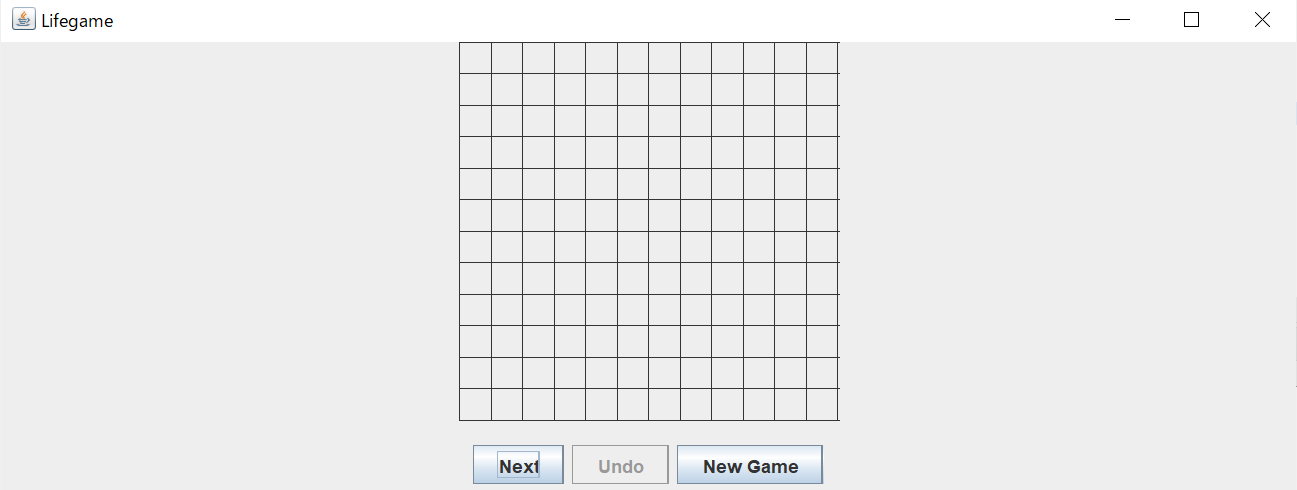
\includegraphics[keepaspectratio, scale=0.3]{wide.png}
      \caption{極端に横に大きくしたときの盤面}
    \end{minipage}
    \begin{minipage}[b]{0.45\linewidth}
      \centering
      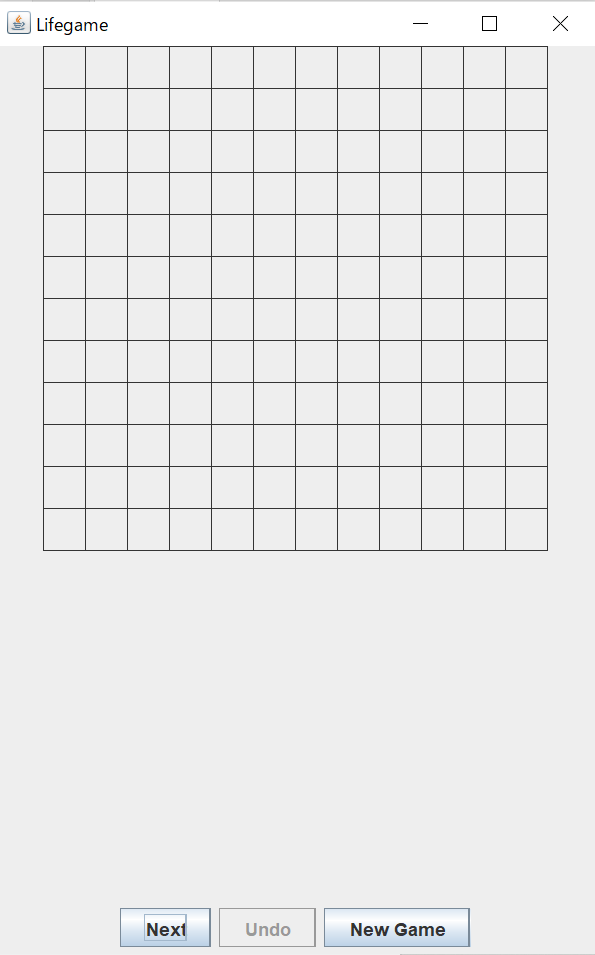
\includegraphics[keepaspectratio, scale=0.3]{height.png}
      \caption{極端に縦に大きくしたときの盤面}
    \end{minipage}
  \end{figure}
  \\上の図のようにウィンドウのサイズが変更されてもセルの形は常に正方形を保つ.具体的な盤面内の座標の計算は実現方法のところで記述する.
\subsubsection{盤面のサイズ変更}
ユーザは盤面のセル数を,該当部のコードを書き換えることで指定することができる.
以下の図4はMainクラス内のコードの一部である.Nは縦のセルの個数,Mは横のセルの個数を表すint型の内部変数である.
\begin{figure}[h]
  \centering
  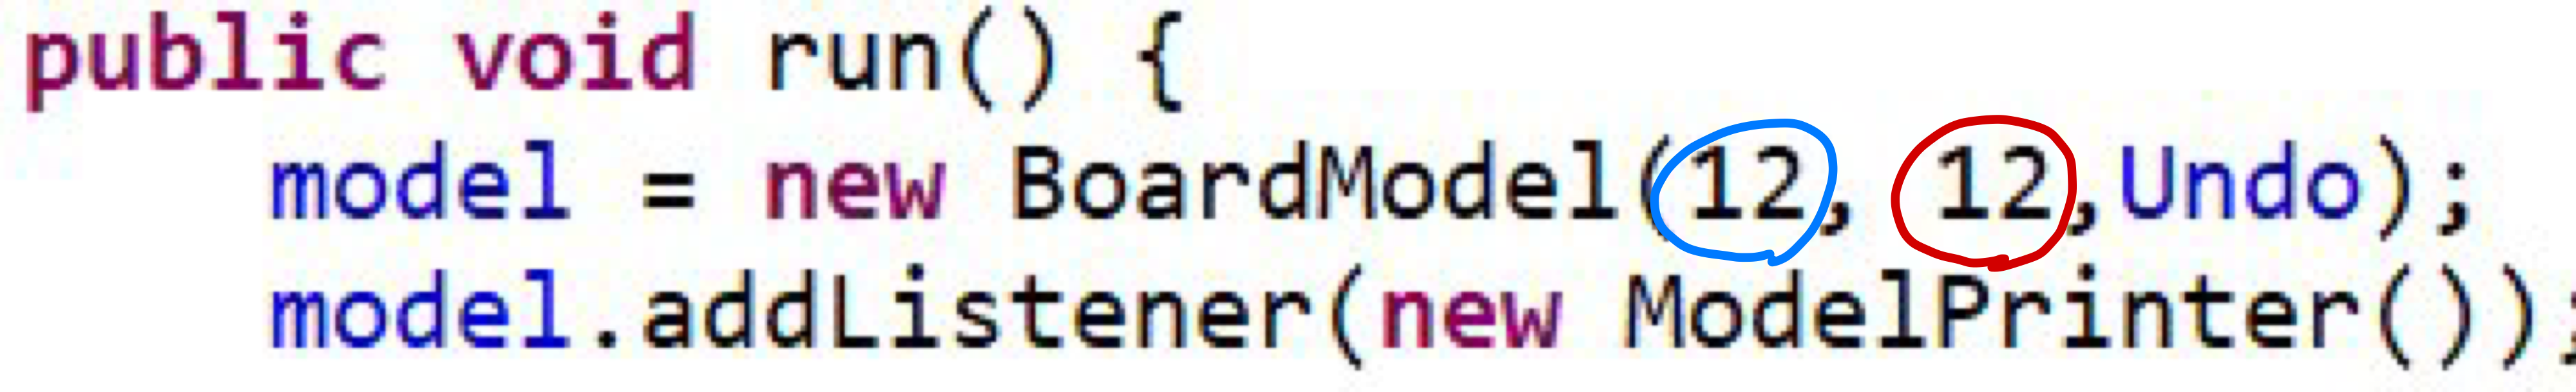
\includegraphics[width=6cm]{code_masu.png}
  \caption{該当部分のコード}
\end{figure}
\\また,変更できる盤面のセル数の最大値は横が282個,縦が123個である.また,最小値は縦も横も1個である.この範囲外の数値をNとMに指定すると"Error"と出力してプログラムを終了する.
以下の図5,6はRUNボタンを押して出力した$12\times12$と$18\times12$の盤面である.
\begin{figure}[htbp]
  \begin{minipage}[b]{0.45\linewidth}
    \centering
    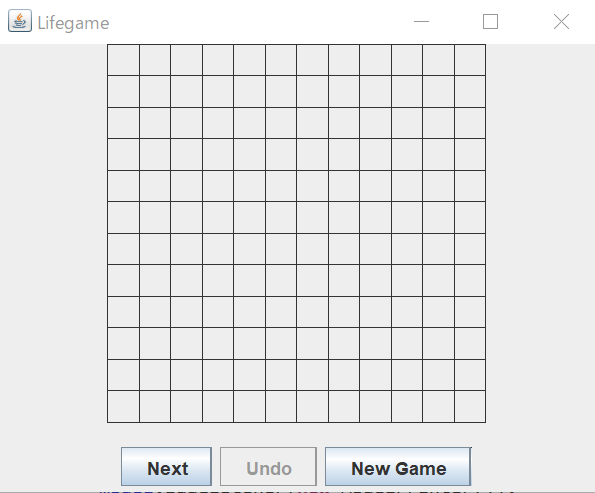
\includegraphics[keepaspectratio, scale=0.4]{panel_normal.png}
    \caption{$12\times12$の盤面}
  \end{minipage}
  \begin{minipage}[b]{0.45\linewidth}
    \centering
    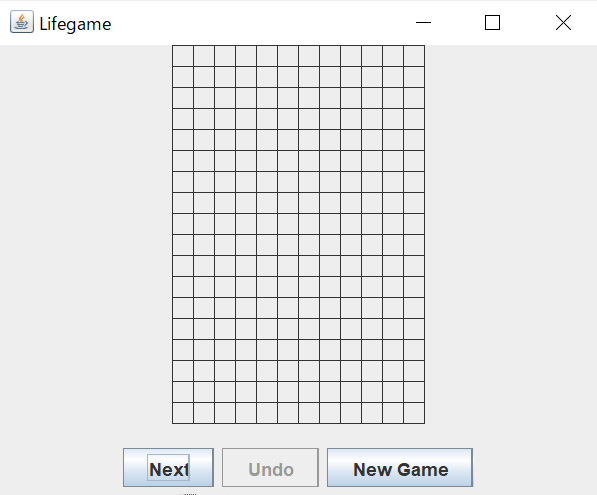
\includegraphics[keepaspectratio, scale=0.4]{1812.png}
    \caption{$18\times12$の盤面}
  \end{minipage}
\end{figure}
\subsection{next,undo,newgameボタン}
ユーザは盤面の下部に表示されるそれぞれのボタンの上にマウスカーソルを移動し左クリックを押し込むことで以下の仕様を満たす処理を実行することができる.
それぞれの処理は左クリックを押し込んで離したときに実行される.
\subsubsection{nextボタン}
nextボタンは最初から押せる状態になっており,ライフゲームの仕様に基づいて世代を一世代進める.具体的には,生きているセルは周りに2または3個の生きているセルがあるとき次の世代でも生きている状態が続き,それ以外の個数であれば次の世代では死んでいる状態となる.また,死んでいるセルは
周りに3個の生きているセルがあるときに次の世代では生きている状態となるがそれ以外の個数であれば次の世代でも死んでいる状態を維持する.また,隣に存在しないセルがある盤面の端のセルに関しては,その存在しないセルを死んでいるセルとして考えた.
以下の図7,8はnextボタンを押して盤面の状態を一世代進めたときの例である.
\begin{figure}[htbp]
  \begin{minipage}[b]{0.45\linewidth}
    \centering
    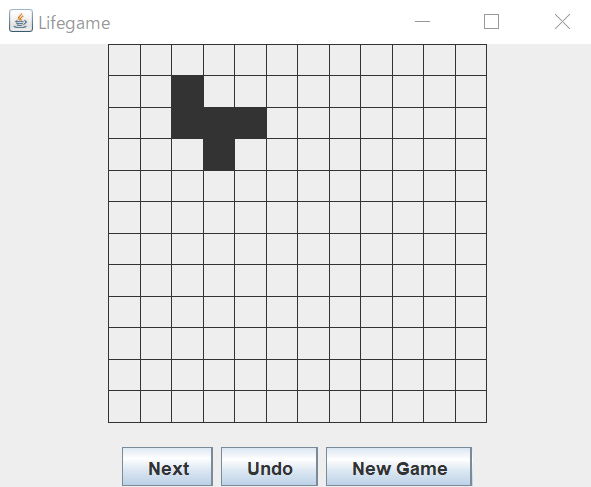
\includegraphics[keepaspectratio, scale=0.35]{before_next.png}
    \caption{nextボタンを押す前の盤面}
  \end{minipage}
  \begin{minipage}[b]{0.45\linewidth}
    \centering
    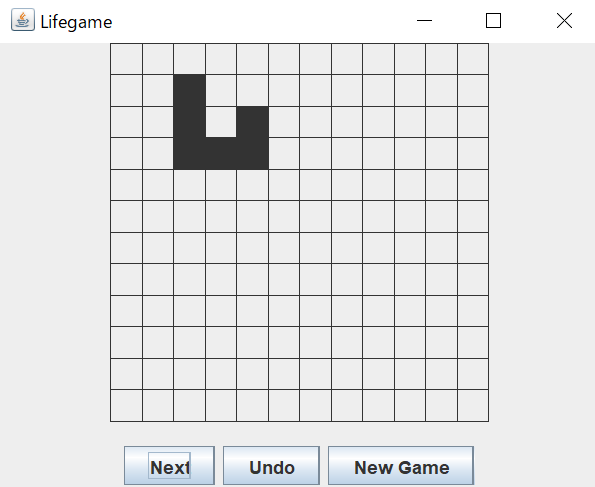
\includegraphics[keepaspectratio, scale=0.35]{after_next.png}
    \caption{nextボタンを押した後の盤面}
  \end{minipage}
\end{figure}
\subsubsection{undoボタン}
undoボタンは最初は色が薄くなって押せない状態になっている.nextボタンを押して盤面の状態を1世代進めるか,マウスカーソルを使って盤面内をクリックまたはドラッグした時に押せるようになる.
最大で32個の状態を記憶することができ,33回以上盤面の状態が変化した場合は直近の32個の盤面の状態を記憶しておく.また,undoが押されると細心の盤面の状態が履歴から消える.
盤面の履歴がこれ以上ない状態まで巻き戻されると再び無効な状態に戻る.したがって,33回盤面の状態が変化した際は,32回undoを押した段階でundoが押せなくなってしまう.
また,盤面の状態の記憶は1セルの状態が変化すると実行されるので,3セル分ドラッグ操作をした場合はその操作で3つの状態が記憶されることになる.
以下の図9はRUNボタンを押したときにUndoボタンが押せなくなっている様子である.
\begin{figure}[h]
  \centering
  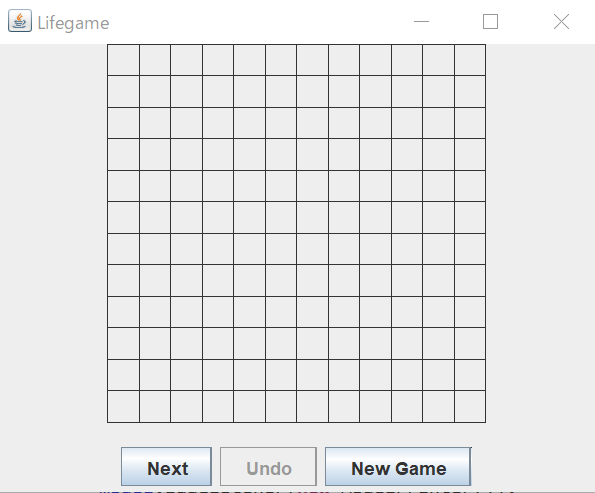
\includegraphics[width=4cm]{panel_normal.png}
  \caption{Undoボタンが押せない様子}
\end{figure}
\\また,以下の図10,11はundoボタンを押して盤面の状態を一世代前に戻したときの例である.
\begin{figure}[htbp]
  \begin{minipage}[b]{0.45\linewidth}
    \centering
    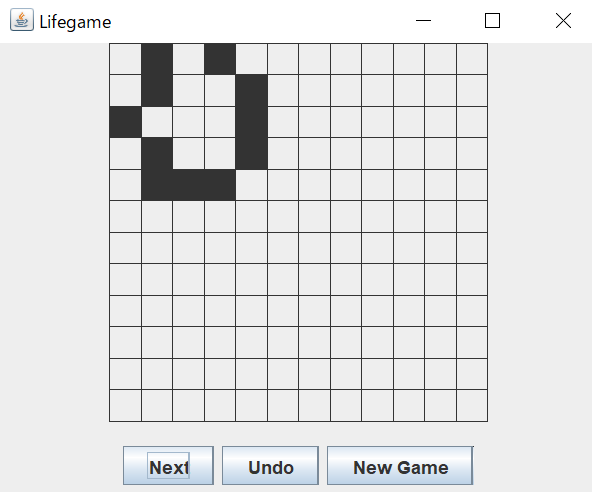
\includegraphics[keepaspectratio, scale=0.35]{before_undo.png}
    \caption{undoボタンを押す前の盤面}
  \end{minipage}
  \begin{minipage}[b]{0.45\linewidth}
    \centering
    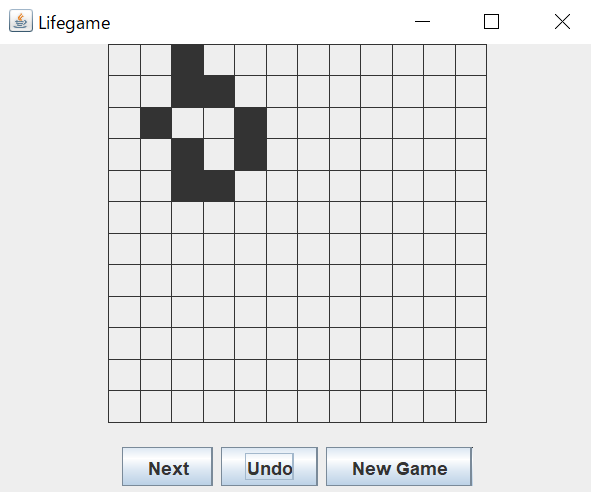
\includegraphics[keepaspectratio, scale=0.4]{after_undo.png}
    \caption{undoボタンを押した後の盤面}
  \end{minipage}
\end{figure}
\subsubsection{newgameボタン}
newgameボタンは最初から押せる状態になっており,ボタンを押すごとに新しく初期化されている盤面を新しいウィンドウで開く.新しく作られたウィンドウはもともとあったウィンドウが作成された位置に作成される.ゲームはそれぞれ
独立しており,片方の盤面の状態を変化させてももう片方の盤面には影響されない.
以下の図12はnewgameボタンを押して新しくウィンドウを開き,片方の盤面にだけマウスカーソルによって状態を変化させた様子である.
\begin{figure}[h]
  \centering
  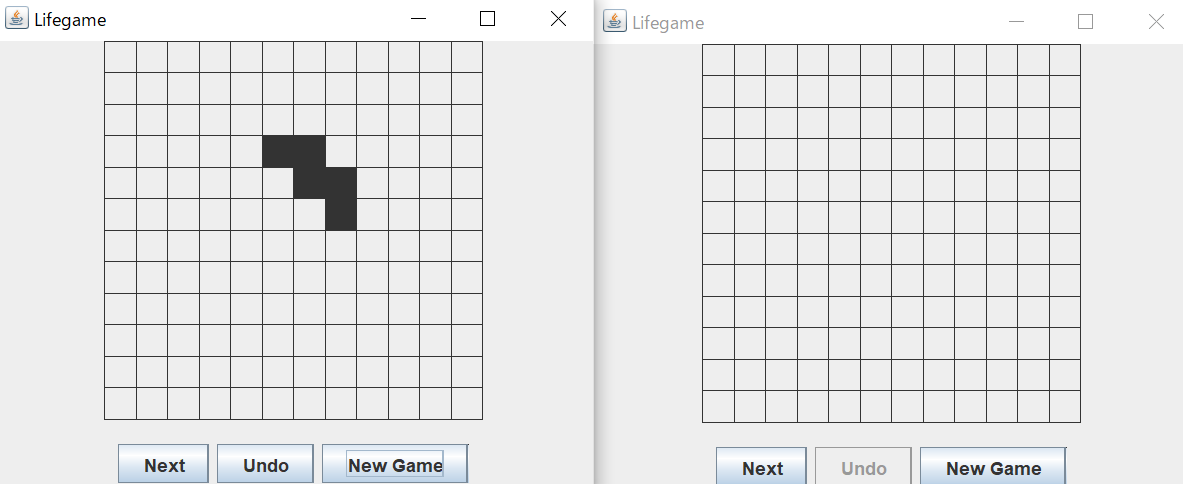
\includegraphics[width=6cm]{newgame.png}
  \caption{newgameボタンを押して片方の盤面だけ変化させた様子}
\end{figure}
\subsection{クリック,ドラッグしたときの処理}
これから記述するクリック操作はマウスカーソルを動かさないで左クリックをすると実行できる.この操作はボタンが押し込まれた瞬間に実行される.
また,ドラッグ操作は左クリックを押し込みながらマウスカーソルを移動させると実行できる.これもクリック操作と同様に,ボタンが押し込まれた瞬間に実行される.
\subsubsection{盤面内のクリック,ドラッグ}
上述のクリック操作により,現在の盤面の状態は反転する.例えば,もともと死んでいる状態のセルをクリックすると生きている状態のクリックに変更し,生きている状態のセルをクリックすると死んでいる状態に変更する.
以下の図13,14は実行例である.この例では(3,4)のセルの状態を反転させている.
\begin{figure}[htbp]
    \begin{minipage}[b]{0.45\linewidth}
      \centering
      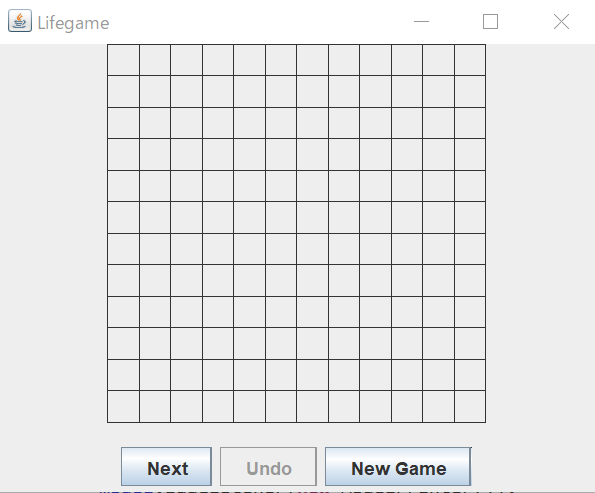
\includegraphics[keepaspectratio, scale=0.4]{panel_normal.png}
      \caption{クリック前の盤面}
    \end{minipage}
    \begin{minipage}[b]{0.45\linewidth}
      \centering
      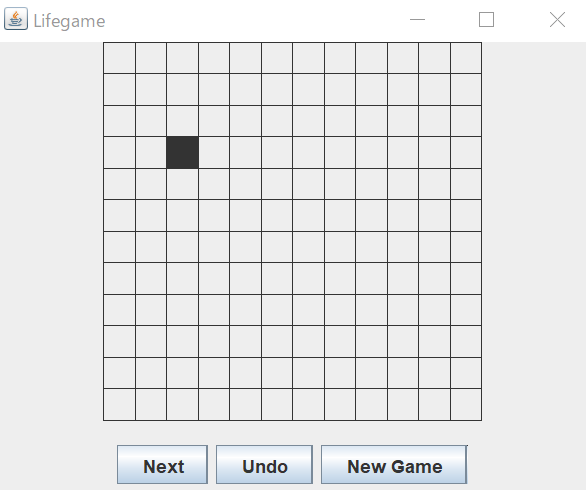
\includegraphics[keepaspectratio, scale=0.4]{panel_click.png}
      \caption{クリックした後の盤面}
    \end{minipage}
  \end{figure}
  \\上述のドラッグ操作により,マウスカーソルがドラッグを開始したセル以外のセルに侵入した
  直後にそのセルの状態が変更される.ただし,同じセル内を移動するだけだと結果としてはクリック操作と同じように押し込んだセルの状態を変更しただけとなる.
  以下の図15,16はドラッグをした時の動作の例である.
  \begin{figure}[htbp]
    \begin{minipage}[b]{0.45\linewidth}
      \centering
      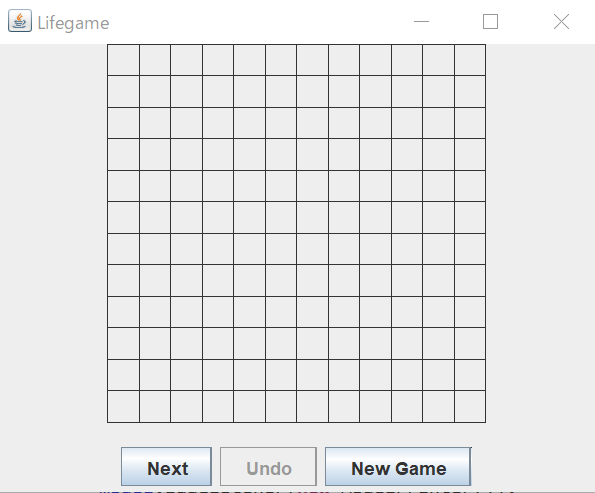
\includegraphics[keepaspectratio, scale=0.4]{panel_normal.png}
      \caption{ドラッグ前の盤面}
    \end{minipage}
    \begin{minipage}[b]{0.45\linewidth}
      \centering
      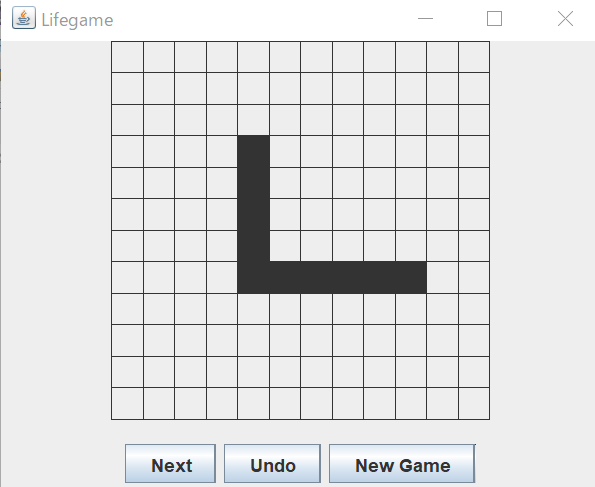
\includegraphics[keepaspectratio, scale=0.4]{panel_drag.png}
      \caption{ドラッグ後の盤面}
    \end{minipage}
\end{figure}
\subsubsection{ドラッグ中にマウスカーソルが盤面以外に移動したときの処理}
盤面外にマウスカーソルを移動させた場合には何も変化が起こらないという仕様にした.また,図17のようにドラッグしながらマウスカーソルを移動させた場合,侵入された盤面の状態のみを変更するので右の図18のように盤面が変更される.
\begin{figure}[htbp]
  \begin{minipage}[b]{0.45\linewidth}
    \centering
    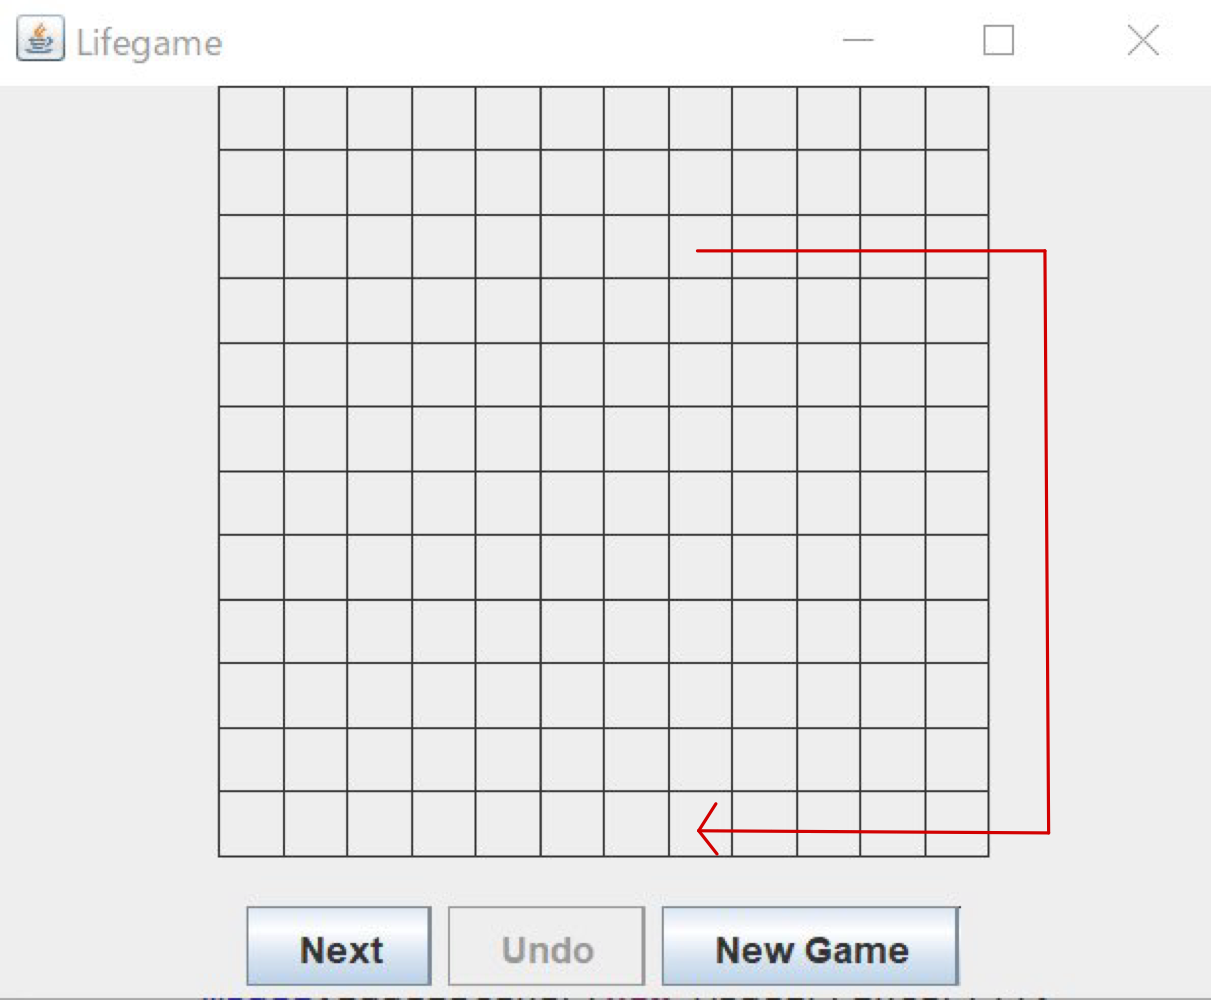
\includegraphics[keepaspectratio, scale=0.1]{tegaki.png}
    \caption{マウスカーソルの動かし方}
  \end{minipage}
  \begin{minipage}[b]{0.45\linewidth}
    \centering
    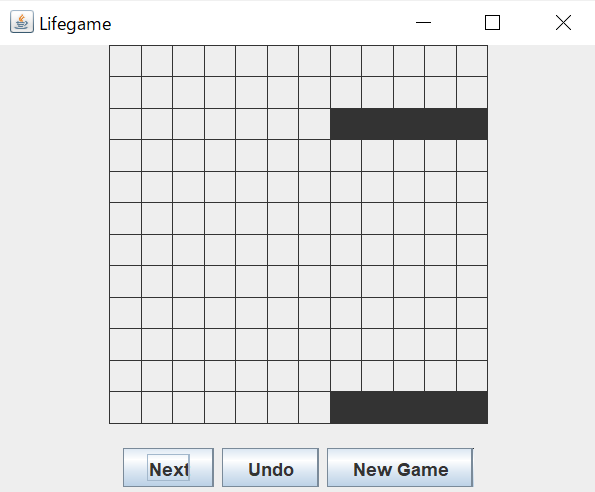
\includegraphics[keepaspectratio, scale=0.4]{after_drag.png}
    \caption{ドラッグ後の盤面}
  \end{minipage}
\end{figure}
\subsubsection{盤面以外をクリックしたときの処理}
盤面以外の場所をクリックした際はドラッグの時と同様に何も起こらないという仕様にした.
\subsubsection{ドラッグ,クリック時のundoボタンの巻き戻し}
1.1.2で記述したundoボタンはクリック,ドラッグ操作による状態の変更も記憶して巻き戻すという仕様とした.ドラッグ操作に関しては,各セル一つずつが状態変化するたびに
新しく盤面が記憶される.

\section{クラスと機能の対応表}
今回作成したライフゲームのプログラムのクラスと機能の対応表は以下の表1のようになる.
\begin{table}[h]
  \centering
  \begin{tabular}{|c|c|}
    \hline
    クラス名&機能\\\hline\hline
    Mainクラス&パネル内の情報の初期設定\\\hline
    BoardModelクラス&盤面の世代更新,巻き戻し処理,盤面の状態変更\\\hline
    Buttonクラス&パネルのボタンが押された時の処理の分類\\\hline
    BoardViewクラス&マウスカーソルによる処理及び盤面の描画\\\hline
  \end{tabular}
  \caption{クラスと機能の対応表}
\end{table}
\subsection{役割分担の方針及びその達成度}
各クラスの役割分担の方針としては,以下の通りになった.
\begin{itemize}
  \item Mainクラス\mbox{}\\
  パネルの情報の初期化をする.
  \item BoardModel\mbox{}\\
  盤面の状態を格納している配列の値の操作を記述する.
  \item Button\mbox{}\\
  ボタンが押された時の処理内容を記述する.
  \item BoardView\mbox{}\\
  マウスカーソルによる状態の変更を記述する.
\end{itemize}
また,その達成度は以下の通りになった.
\begin{itemize}
  \item Mainクラス\mbox{}\\
  このクラスは方針で挙げた内容を実装することができた.
  \item BoardModel\mbox{}\\
  このクラスは方針で挙げた配列の値の処理のほかに盤面の状態を記憶する処理を行った.方針とは少し違った内容を含めてしまったが
  もともとの目標であった機能を実装することはできた.
  \item Button\mbox{}\\
  このクラスは方針で挙げた内容を実装することができた.
  \item BoardView\mbox{}\\
  このクラスは方針で挙げた内容を実装することができた.
\end{itemize}
\section{各機能実装方法}

\subsection{画面の表示項目}
今回のライフゲームでの画面の表示項目とその実装方法は以下のとおりである.
\begin{itemize}
  \item 盤面
  \item next,undo,newgameボタン
\end{itemize}

\subsection{状態の更新に連動して画面表示の更新方法}
今回のライフゲームでの画面表示が変更されるのは以下のような場合である.
\begin{itemize}
    \item nextボタンやundoボタンによる盤面の更新及び巻き戻し
    \item マウスカーソルによる盤面の状態の変更
\end{itemize}
これらの処理が行われた後に盤面が再描写されるための処理について記述する.\\
以下のListing1からListing4のコードはこの処理を実装するためにそれぞれのクラスから必要な個所のみを抜粋したコードである.
\begin{lstlisting}[caption=BoardListenerインターフェース,label=fuga]
    public interface BoardListener {
	    public void updated(BoardModel m);
    }
\end{lstlisting}
\begin{lstlisting}[caption=Mainクラス,label=fuga]
    model.addListener(new BoardView(model));
\end{lstlisting}
\begin{lstlisting}[caption=BoardViewクラス,label=fuga]
    public BoardView(BoardModel model) {
		this.model = model;
		this.addMouseListener(this);
		this.addMouseMotionListener(this);
		model.addListener(this);
	}
    @Override
	public void updated(BoardModel model) {
		this.repaint();
	}
\end{lstlisting}
\begin{lstlisting}[caption=BoardModelクラス,label=fuga]
    private ArrayList<BoardListener> listeners;

    public BoardModel(int c,int r,JButton undoButton) {
		listeners = new ArrayList<BoardListener>();
	}

    public void changeCellState(int x,int y) {
		this.fireUpdate();
	}

    public void addListener(BoardListener listener) {
		listeners.add(listener);
	}
	
	private void fireUpdate() {
		for(BoardListener listener:listeners) {
			listener.updated(this);
		}
	}
\end{lstlisting}
listing1の2行目において,BoardListenerインターフェースにはupdatedクラスが呼び出されている.このupdatedクラスの処理内容はlisting3の8から10行目のように,上で挙げた盤面が更新されるための
処理を実装するクラス内に記述されている.
listing2のコードにより,BoardListenerインターフェースをimplementしたクラスのオブジェクトをlisting4の10から12行目のaddListenerクラスで可変長配列
listenersに登録している.これを行うことで,盤面を変更する各操作が実行されるたびにlisting4の9から12行目のChangeCellStateメソッドが呼び出されて盤面を変更し,その後で18から21行目のfireupdatedメソッドが
呼び出されてrepaintが実行される.これにより,すべての盤面の変更が起こったときにlistenersに登録されたオブジェクトを使ってBoardListenerを介して盤面の再描画が実行される.


\subsection{巻き戻しのための盤面の記憶}
巻き戻しのための盤面の記憶に関する処理はBoardModelクラスに記述した.盤面の情報は可変長配列を持つリスト型であるArraylistを使用し,変数名はHistoryとした.
\subsubsection{nextによる盤面の状態の変更の記憶}
以下のListing5はBoardModelクラスのnextメソッドの一部である.
\begin{lstlisting}[caption=nextメソッドの一部,label=fuga]
    boolean[][] currentBoard = new boolean[rows][cols];
    for (int i = 0; i < rows; i++) {
        System.arraycopy(cells[i], 0, currentBoard[i], 0, cols);
    }
    if(counter!=32) {
        counter++;
        History.add(copiedcells);
    }else {
        History.remove(0);
        History.add(copiedcells);
    }
\end{lstlisting}
counterはHistoryに記憶されている状態の数を表すint型の変数で0に初期化されている.counterはメンバであるためcounterの値はほかのメソッドにも共有される.記憶されている状態の数が32個以下ならcounterの値を1インクリメントしてからaddメソッドを使ってHistoryに
状態を記憶し,32個ならHistoryに記憶されている一番古い状態を削除してからaddメソッドを使って現在の状態を新しく記憶している.また,copiedcellsはlifegameの仕様に基づいて一世代進めたあとの盤面の状態を表す二次元配列である.
これは現在の盤面の状態を表す二次元配列cellsのすべての要素をコピーしたものである.copiedcellsを使用している理由としては,次の世代へ進めたときに各セルが生きているかはセルの周りに生きているセルが何個存在するかで決定されるので全てのcellsの要素に参照している途中でcellsの状態を変えてしまうと
周りに存在する生きているセルの数が変化してしまうためである.
\subsubsection{undoによる盤面の状態の変更の記憶}
以下のListing6はBoardModelクラスのundoメソッドの一部である.
\begin{lstlisting}[caption=undoメソッドの一部,label=fuga]
    History.remove(counter);
    counter--;
    cells = History.get(counter);
\end{lstlisting}
まず一番最新の状態をHistoryから削除し,そのあとにcounterを1デクリメントする.これによりundoが押された際に記憶されていた状態が1つ減少する.その後現在の状態を表す二次元配列cells
にデクリメントした後のcounterがさすHistoryの最新の状態,即ちundoを押したときの直前の状態を格納する.
\subsubsection{マウスカーソルによる盤面の状態の変更の記憶}
以下のListing7はBoardModelクラスのchangeCellStateメソッドの一部である.
\begin{lstlisting}[caption=changeCellStateメソッドの一部,label=fuga]
    boolean[][] currentBoard = new boolean[rows][cols];
    for (int i = 0; i < rows; i++) {
        System.arraycopy(cells[i], 0, currentBoard[i], 0, cols);
    }
    if(counter!=32) {
        counter++;
        History.add(currentBoard);
    }else {
        History.remove(0);
        History.add(currentBoard);
    }
\end{lstlisting}
マウスカーソルによる盤面の状態はどのセルの状態を変更すればよいかを特定してから
changeCellStateを呼び出して実際に盤面の状態を格納しているcellsを変更する.二次元配列であるcurrentBoardを用意して変更後の盤面の状態を2から4行目でコピーする.
その後counterの値が32以下ならcounterの値を1インクリメントしてからaddメソッドを使ってHistoryに
状態を記憶し,32個ならHistoryに記憶されている一番古い状態を削除してからaddメソッドを使って現在の状態を新しく記憶している.
addした配列がcellsではなくcurrentBoardである理由は,cellsを格納してしまうと参照の追加になり,cellsが変更されるとHistoryに追加されているほかのオブジェクトも同じように変更されてしまうためである.
ゆえに一時的にcellの内容を別の二次元配列にコピーして参照の追加となることを避けた.
\subsection{undoによる巻き戻しが可能かどうかの判定}
undoは盤面を生成したときMainメソッド内でsetEnabledメソッドを使って押せないように初期化されている.undoによる巻き戻しが可能となるのは仕様でも説明した通り
nextボタンによる世代の更新かマウスカーソルによる盤面の状態の変更が行われた時である.
\begin{itemize}
    \item nextボタンによって世代更新が行われた時,3.2.1で記述したようにcounterの値が更新された回数だけインクリメントされる.これを利用してBoardModelメソッド内にisUndoableメソッドを作成した.
    このメソッドはcounterの値が0より大きいときはtrueを,0のときはfalseを返す.以下のListing8のコードはButtonクラス内のnextボタンとundoボタンが押された時に実行される処理である.
    \begin{lstlisting}[caption=nextボタン及びundoボタンを押したときに実行される処理,label=fuga]
        case 1:
            boardModel.next();
            undoButton.setEnabled(true);
            break;
        case 2:
            if(boardModel.isUndoable()) {
                boardModel.undo();
                if(!boardModel.isUndoable()) {
                    undoButton.setEnabled(false);
                }
            }
            break;
    \end{lstlisting}
    1から4行目のように,nextボタンが押された時にはnextメソッドを呼び出して盤面の世代を更新してからsetEnabledメソッドでundoボタンを押せるようにしている.また,6から11行目のように
    isUndoableの返り値がtrueの時はundoメソッドを呼び出して盤面の世代を一つ戻した後に再びisUndoableメソッドを呼び出して返り値がfalseであればsetEnabledメソッドでundoボタンを押せなくしている.
    これは,undoメソッドによって世代を戻したときにHistoryが空になったことをすぐに確認するためである.これを実装することでUndoボタンが履歴がなくなった時に押せなくなることを実現できる.
    \item マウスカーソルによって盤面に変更が加えられたときは仕様で述べた通り,セルの状態が一つでも変わるとそれが一つの盤面の状態として記憶される.3.2.3で記述した通り,マウスカーソルで状態が変更されると
    changeCellStateメソッドが呼び出されるのでこのメソッドが呼び出された時にsetEnabledメソッドでundoボタンを押せるようにすれば巻き戻しを可能にすることが実現できる.
\end{itemize}

\subsection{セルの境界線の位置を計算する方法}
以下の表2は計算するために使用した変数名と表す内容である.
\begin{table}[h]
\centering
\begin{tabular}{|c||c|}
    \hline
    変数名 & 変数があらわす内容\\
    \hline\hline
    M & 盤面の横のセル数\\\hline
    N & 盤面の縦のセル数\\\hline
    width & パネルの横幅\\\hline
    height & パネルの縦幅\\\hline
    masu & 盤面に描写する正方形のマスの一辺の長さ\\\hline
\end{tabular}
\caption{計算式中の変数名とその内容}
\end{table}
\\盤面のセルの境界線の位置は以下のような手順で盤面の境界線の位置は計算される.
\begin{enumerate}
    \item 現在のwidthとheightから,masuを決定する.具体的には以下のような不等式が成り立つかどうかについて考える.
    \begin{align}
        \frac{height\times\frac{99}{100}}{N} > \frac{width}{M+2}
    \end{align}
    左辺はheightの99\%の大きさをN等分した時の長さを調べている.これは,heightの99\%の長さを考えないと盤面の一番下の横線が表示されないことがあるという問題を解決するための処理である.
    右辺はwidthをM+2等分したときの長さを調べている.これは,パネルの中央に盤面を配置するための処理である.(1)が成り立った時はパネルが縦に長い状態であると判断して
    \begin{align}
        masu=\frac{width}{M+2}
    \end{align}
    とし,(1)が成り立たなかったときはパネルが横に長い状態であると判断して
    \begin{align}
        masu = \frac{height\times\frac{99}{100}}{N}
    \end{align}
    となるようにした.
    \item 次に,盤面の開始位置を決定する.縦軸の開始位置はy座標が0からである.x座標の開始位置はパネルの中央に盤面を配置するために,以下のような数式の値を開始位置とする.
    \begin{align}
        \frac{width-masu\times M}{2}
    \end{align}
    この数式はパネルの横幅から盤面を表示している部分の長さを引いた長さを二等分した値になる.これにより,盤面を描写していない部分の横幅が同じ長さとなっている.
    \item ユーザが指定したセル数分だけ縦軸と横軸を描画する.それぞれのセルの一片の長さは(2)または(3)の値である.
\end{enumerate}
\clearpage
\subsection{マウスカーソルの座標からセルの座標を計算する方法}
以下の表3は計算するために使用した変数名と表す内容である.
\begin{table}[h]
    \centering
    \begin{tabular}{|c||c|}
        \hline
        変数名 & 変数があらわす内容\\
        \hline\hline
        M & 盤面の横のセル数\\\hline
        N & 盤面の縦のセル数\\\hline
        width & パネルの横幅\\\hline
        height & パネルの縦幅\\\hline
        masu & 盤面に描写する正方形のマスの一辺の長さ\\\hline
        x & マウスカーソルがある場所のx座標\\\hline
        y & マウスカーソルがある場所のy座標\\\hline
        masu\_x & 0で初期化されており,マウスカーソルが現在存在するセルの左上の頂点のx座標\\\hline
        masu\_y & 0で初期化されており,マウスカーソルが現在存在するセルの左上の頂点のy座標\\\hline
        StateX & マウスカーソルが現在存在するセルの左上の頂点のx座標\\\hline
        StateY & マウスカーソルが現在存在するセルの左上の頂点のy座標\\\hline
        i &for文を使う際のカウンタ\\\hline
        j &for文を使う際のカウンタ \\\hline
    \end{tabular}
    \caption{計算式中の変数名とその内容}
    \end{table}
\\3.4の表2の変数と同じ変数名のものは値も同じである.以下のような流れでマウスカーソルがある位置のセルの座標はクリックとドラッグで異なる方法で計算される.
\begin{enumerate}
  \item 盤面外にマウスカーソルがある状態でクリックやドラッグがされると何もしないようにするためにxとyが以下の条件式を満たしているか確認する.
  \begin{align}
      x < \frac{width-masu\times M}{2} \quad or \quad x> \frac{width+masu\times M}{2}\quad or \quad y > masu\times (N)
  \end{align}
  これらの3つの不等式の一番左の不等式はマウスカーソルのx座標が盤面よりも左側にあるとき真になる.真ん中はマウスカーソルのx座標が盤面よりも右側にあるとき真になる.
  一番右の不等式はマウスカーソルのy座標が盤面よりも下側にある時に真になる.そしてこれら3つの不等式は全てorとしているのでこれらのうちの1つでも真になれば盤面外にマウスカーソルがあるという判定になる.
  \item for文を使って今現在のマウスカーソルが存在する座標のセルのy座標を特定する.このとき,特定するための条件式は以下のようになる.
  \begin{align}
    y  \geqq  i*masu \quad and \quad y  < (i+1)*masu
  \end{align}
  この条件式が真になった時のiの値が求めるセルのy座標となる.このとき,andの左側の不等式にイコールが入っていることから,セルの境界線の上側はそのセル内に含まれるという判定になる.
  \item y座標を特定してから再びfor分を使って今現在のマウスカーソルが存在する座標のセルのx座標を特定する.このとき,特定するための条件式は以下のようになる.
  \begin{align}
    x \geqq \frac{width-masu \times M}{2}+masu*j \quad and \quad x< \frac{width-masu \times M}{2} + masu*(j+1)
  \end{align}
  この条件式が真になった時のjの値が求めるセルのx座標となる.このとき,andの左側の不等式にイコールが入っていることから,セルの境界線の左側はそのセル内に含まれるという判定になる.
\end{enumerate}

\subsection{新しいウィンドウを開く}
以下のListing9はButtonクラスのActionPerformedメソッドの一部で,listingはMainメソッドのコードの一部である.
\begin{lstlisting}[caption=Buttonクラスの一部,label=fuga]
    case 3:
    SwingUtilities.invokeLater(new Main());
    break;
\end{lstlisting}
\begin{lstlisting}[caption=Buttonクラスの一部,label=fuga]
    public static void main(String[] args) {
          SwingUtilities.invokeLater(new Main());
      }
\end{lstlisting}
Listing9の2行目は空の盤面を作り新しいウィンドウを開くという処理を表しており,ゲームが開始された時に実行されてパネルが一つ生成される.それと同じ処理をListing10の2行目に記述した.  この処理は
Newgameボタンが押された時に実行されるため,Newgameボタンを押したときの処理を実現できた.
\clearpage
\section{プログラミングの講義・演習で学習したこと}
\subsection{演習で試すまでに理解できなかったこと}
私はこの授業を通して継承とインターフェースについて深く学ぶことができたと考えている.javaの基本的な構文や,オブジェクトというものの存在など
は講義資料や参考図書の教材を読むことで理解することができたが,この二つだけは実際にプログラムを書いて動かしてみないと理解することができなかった.
特に,インターフェースはライフゲームのプログラム中のAddListenerで使用したが理解するのにかなり時間がかかってしまった.
\subsection{同一のプログラムを現段階で書き直すときに変更する点}
今回のプログラムではBoardModelクラスで盤面の状態を表す配列の世代を進めたり戻したりする処理と,盤面の状態の記憶を実現した.
しかし,オブジェクト指向プログラミングの観点からなるべく処理内容は細分化したほうが今後の大人数での開発にも適していることから,先ほど挙げた二つの処理は分割して別々のクラスに記述すべきだと考えた.
具体的にはBoardModelクラスには盤面の状態を格納する配列の値を変更する処理をそのまま書いて,新たにHistoryクラスを作成してそこに盤面の記憶に関する処理を書くべきだと考えた.\\
また,BoardViewクラスに関しても,マウスカーソルによる変更するセルの座標の取得と盤面の描写という二つの役割が同じクラス内に記述されているので同様の理由から別々のクラスに記述すべきだと考えた.
具体的にはBoardViewクラスには盤面の描写に関する処理をそのまま記述し,新たにMouseクラスを作成してドラッグやクリックが行われた時の処理を記述すればよいと考えた.
したがって,新たに作成するクラスの役割分担表は以下の表4ようになる.
\begin{table}[h]
  \centering
  \begin{tabular}{|c|c|}
    \hline
    クラス名&機能\\\hline\hline
    Mainクラス&パネル内の情報の初期設定\\\hline
    BoardModelクラス&盤面の世代更新,巻き戻し処理,盤面の状態変更\\\hline
    Historyクラス&盤面の状態の記憶\\\hline
    Buttonクラス&パネルのボタンが押された時の処理の分類\\\hline
    Boardlistenerインターフェース&盤面の情報\\\hline
    BoardViewクラス&盤面の描画\\\hline
    Mouseクラス&マウスカーソルによる処理\\\hline
  \end{tabular}
  \caption{クラスと機能の対応表}
\end{table}
<<<<<<< HEAD



\subsection{拡張機能}


\subsubsection{実現方法}


\section{プログラミングの講義・演習で学習したこと}
今回のプログラミング
=======
>>>>>>> afedfd0cb722702594fd296fbde40408fa722e25
\end{document}